\chapter*{Abstract}
\phantomsection
\addcontentsline{toc}{chapter}{Abstract}%
\markboth{Abstract}{Abstract}%
In the aerospace industry, an ongoing demand exists for lighter aerostructures, motivated by the imperative to enhance fuel efficiency and overall performance. For that reason, the aerospace sector is currently witnessing two innovative shifts: the transition to hydrogen-powered and electric planes, directing engineering efforts toward cleaner and more sustainable aviation technologies. These changes offer opportunities to deviate from the classic tube-and-wing configuration and explore inventive concepts like the flying wing or transonic truss-braced wings. One promising approach to meet these requirements is the utilization of lattice structures. These structures not only offer ultralight properties but also modularity. Modular designs bring numerous advantages, including the ability to assemble large structures from smaller and easier-to-manufacture repeating modules, on-field reparability, and rapid assembly for temporary structures.
The objective of this thesis is to develop a design and optimization algorithm for ultralight and modular aerostructures. In the initial phase, we reviewed existing literature to identify the most suitable algorithm basis for optimizing monolithic (non-modular) structures. After a thorough comparison, we selected the Truss Topology Optimization (TTO) approach, an optimization method based on the use of bars as the discretizing element of the structure. However, the classic TTO formulation has limitations, such as the inability to address buckling constraints, consider multiple load cases, and ensure mechanical compatibility. To overcome these challenges, we proposed an innovative two-step optimization algorithm. In this approach, a relaxed problem is utilized to generate an initial solution, serving as the starting point for the optimization using a complete formulation.
The second part of the thesis focuses on adapting the proposed monolithic formulation to incorporate modular constraints. Initially, the emphasis is on optimizing the topology of a fully modular structure, where a single module is repeated throughout the entire design. We evaluate how hyperparameters, such as the number of subdomains and module complexity, affect the mechanical performance of the structure. Subsequently, we delve into a more complex scenario, optimizing multiple module topologies and their layout within the structure. This is achieved through a Discrete Material Optimization (DMO) approach, employing a gradient-based optimizer.
By addressing the challenges of lightweight design and modularity in aerostructures, this research aims to contribute to the ongoing evolution of aerospace technologies and advance the efficiency and performance of future aircraft.


\newpage
\chapter*{Introduction}
\phantomsection
\addcontentsline{toc}{chapter}{Introduction}
\markboth{Introduction}{Introduction}%
\glsresetall % reset glossary



\textit{Scientists study the world as it is,}\\
\textit{Engineers create the world that never has been.} \vspace{5pt} \\
--- Theodore von K\'arm\'an \\

\section*{Towards lighter structures}

In the aerospace industry, an ongoing demand exists for lighter aerostructures, motivated by the need to enhance fuel efficiency and overall performance. This emphasis on lighter structures and materials not only reduces operational costs for airlines but also aligns with a broader commitment to sustainability, mitigating fuel consumption and carbon emissions. Furthermore, the aerospace sector is currently witnessing two innovative shifts: the transition to hydrogen-powered and electric planes, directing engineering efforts toward cleaner and more sustainable aviation technologies. These changes offer opportunities to deviate from the classic tube-and-wing configuration and explore inventive concepts like the flying wing \gls{bwb}, in which the fuselage and the wing blend to form an aircraft in which the fuselage, widened and integrated into the wing, also contributes significantly to the lift. Another explored configuration is the use of transonic truss-braced wings, with the goal of direct reduction in the aerodynamic drag by using a \gls{har} strut-braced wing configuration (see examples in \figref{fig:01_concepts}). Regardless of the specific configuration, a highly probable shared goal is the necessity to design lightweight dry wings—\ie, with no fuel tanks inside—with high aspect ratios and thin profiles.

\begin{figure*}
    \hspace*{\fill}
    \subcaptionbox{}{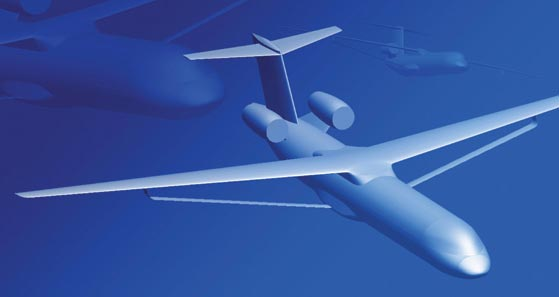
\includegraphics[height=4.3cm]{figures/01_intro/albatros-1.jpg}}
    \hfill
    \subcaptionbox{}{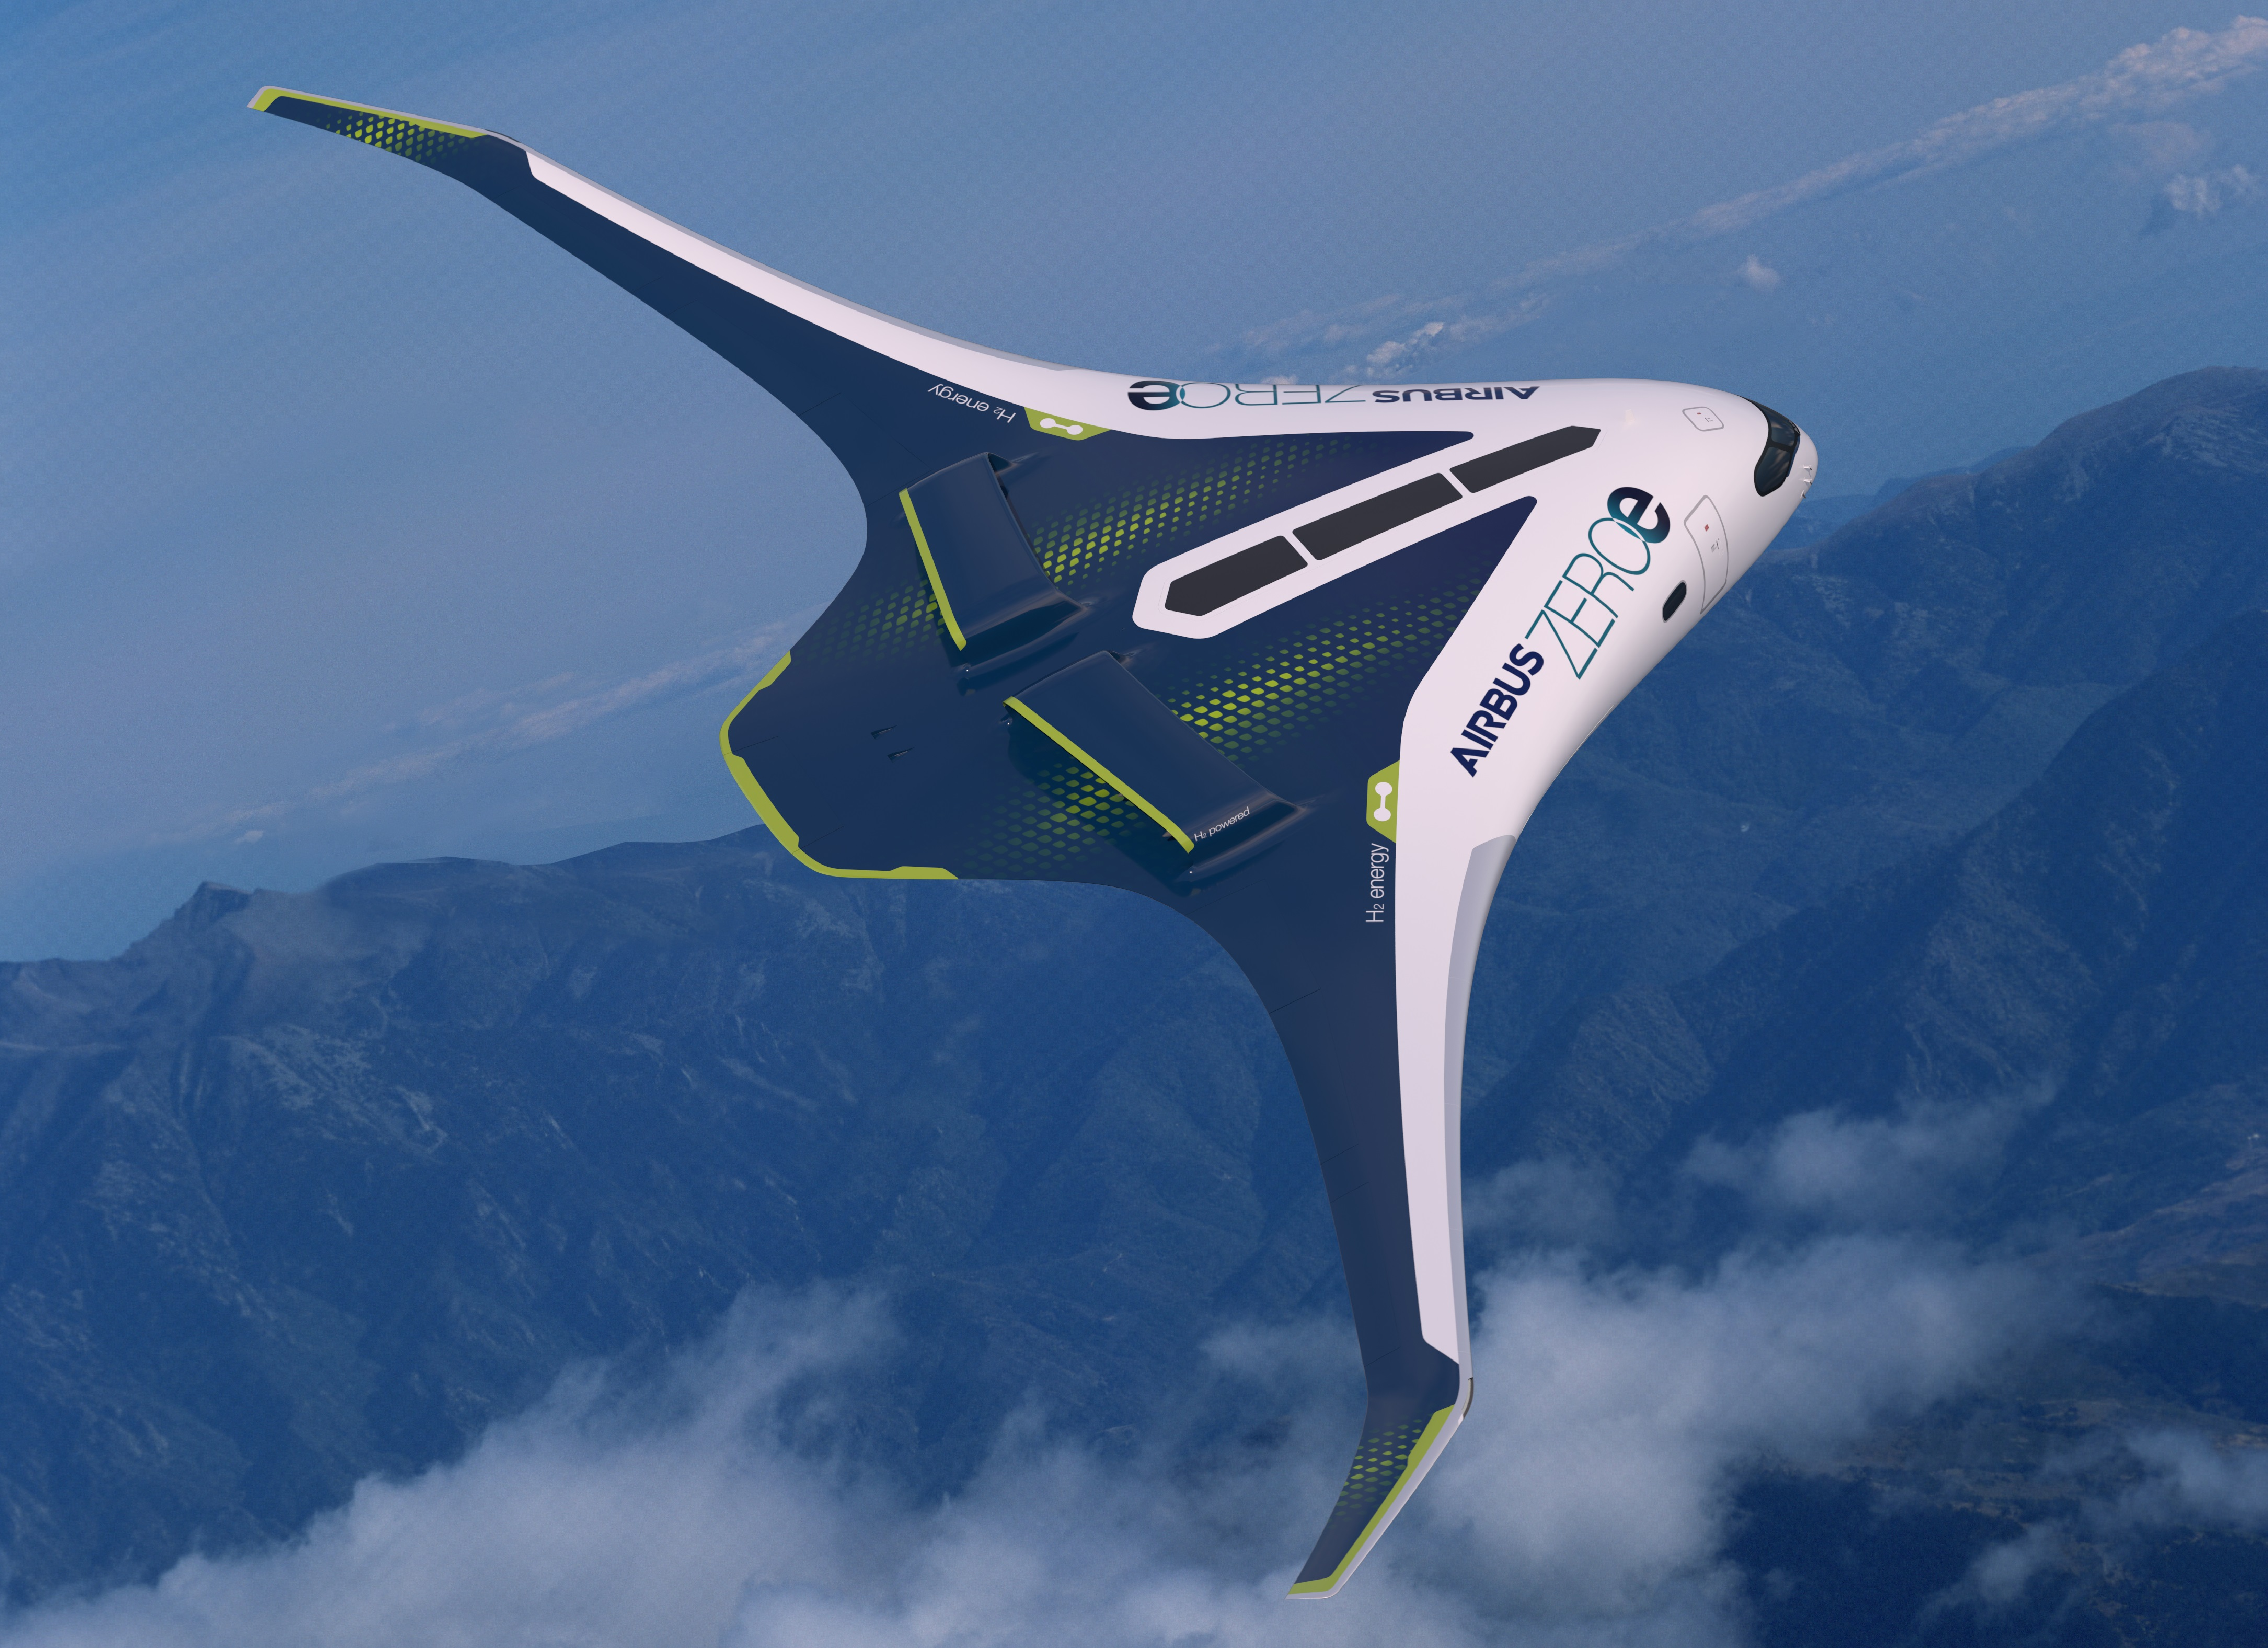
\includegraphics[height=4.3cm]{figures/01_intro/pm_38_529_529759-gml5anffhc.jpg}}
    \hspace*{\fill}
    \caption{(a) The transonic truss-braced wing called ALBATROS by ONERA \cite{carrier_investigation_2012,carrier_multidisciplinary_2021}; (b) the \acrfull{bwb} zero-e demonstrator by Airbus \cite{noauthor_airbus_2021}.}
    \label{fig:01_concepts}
\end{figure*}

Lattices emerge as a promising solution to fulfill these requirements. These structures consist of interconnected elements resulting in an arrangement of material and void spaces, recognized for their remarkable strength-to-weight ratio. Depending on their scale, lattice structures are categorized into two main types: lattice materials and lattice structures. Lattice materials, prevalent in research, are typically fabricated using additive manufacturing techniques and are primarily used to create individual structural components. Conversely, lattice structures, due to their larger size, are impractical to manufacture using additive methods alone. Instead, they are assembled from smaller components to form larger structures. The process of going from materials to structures is not only accompanied by a change in manufacturing processes but also an evolution in the issue of connections \ie, moving from the problem of connecting the structural component made of lattice material to its environment, to the problem of linking the constituent elements of the lattice structure.

When lattice structures present a repetitive pattern, they not only possess the inherent ultralight properties typical of such structures but also provide the advantages of modularity. Modular lattices offer numerous benefits, including the ability to construct large structures using smaller, more readily manufactured repeating modules (see \figref{fig:01_fab}a). Other notable properties include on-field reparability, improved damage resistance, fast assembly for temporary structures, and possibility to repurpose the repetitive components compared to conventional monolithic material systems \sidecite{belvin_space_2016}. Additionally, recent research opens up the possibility of a fully robotic assembly phase, permitting faster and more reliable assembly (see \figref{fig:01_fab}b). These features are crucial to assess whether lattice structures can challenge the classic composite materials in aerospace applications.

\begin{figure}
    \hspace*{\fill}
    \subcaptionbox{}{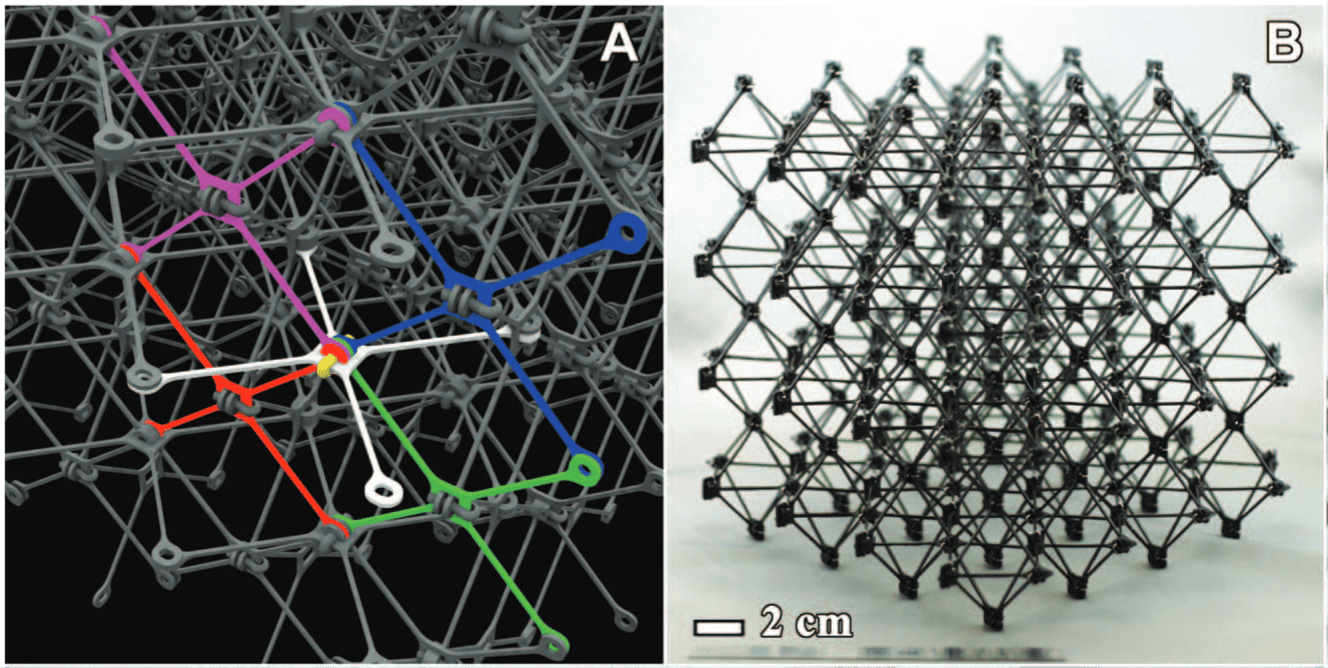
\includegraphics[height=3.5cm]{figures/01_intro/assembly.png}}
    \hfill
    \subcaptionbox{}{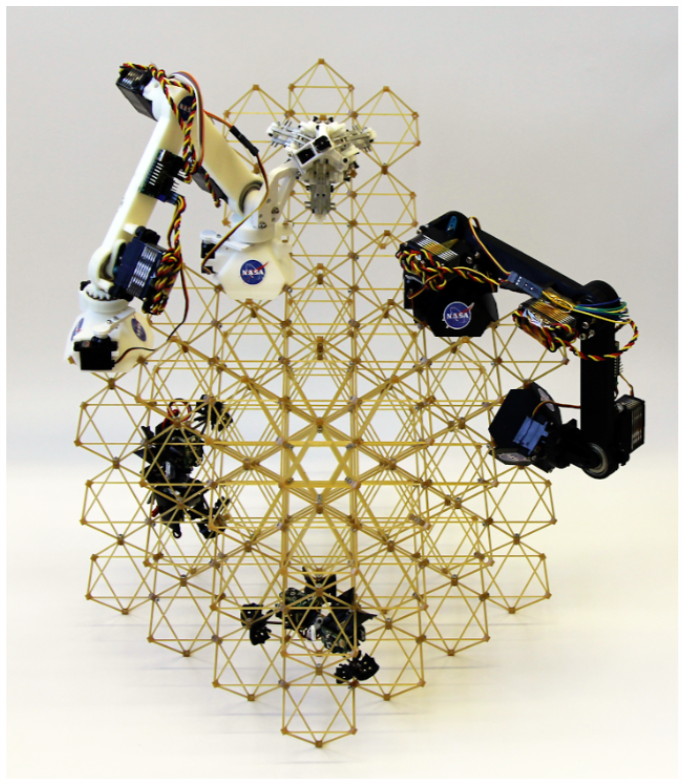
\includegraphics[height=3.5cm]{figures/01_intro/fab.png}}
    \hspace*{\fill}
    \caption{Modular lattice structures present multiple beneficial properties that could be applied to the aerospace domain; (a) small two-dimensional components are reversibly assembled to build large three-dimensional structures \cite{cheung_reversibly_2013}; (b) the assembly phase of modular lattice structures is done by fully robotic means in the NASA's Automated Reconfigurable Mission Adaptive Digital Assembly Systems (ARMADAS) project \cite{costa_algorithmic_2020}.}
    \label{fig:01_fab}
\end{figure}

Given these beneficial properties, ONERA, the French aerospace research agency, initiated the STARAC research project to investigate modular lattice structures more comprehensively (see \figref{fig:01_starac}). This thesis is conducted within this research effort, in a unit dedicated to developing design and optimization methods for such structures.

\begin{marginfigure}
    \centering
    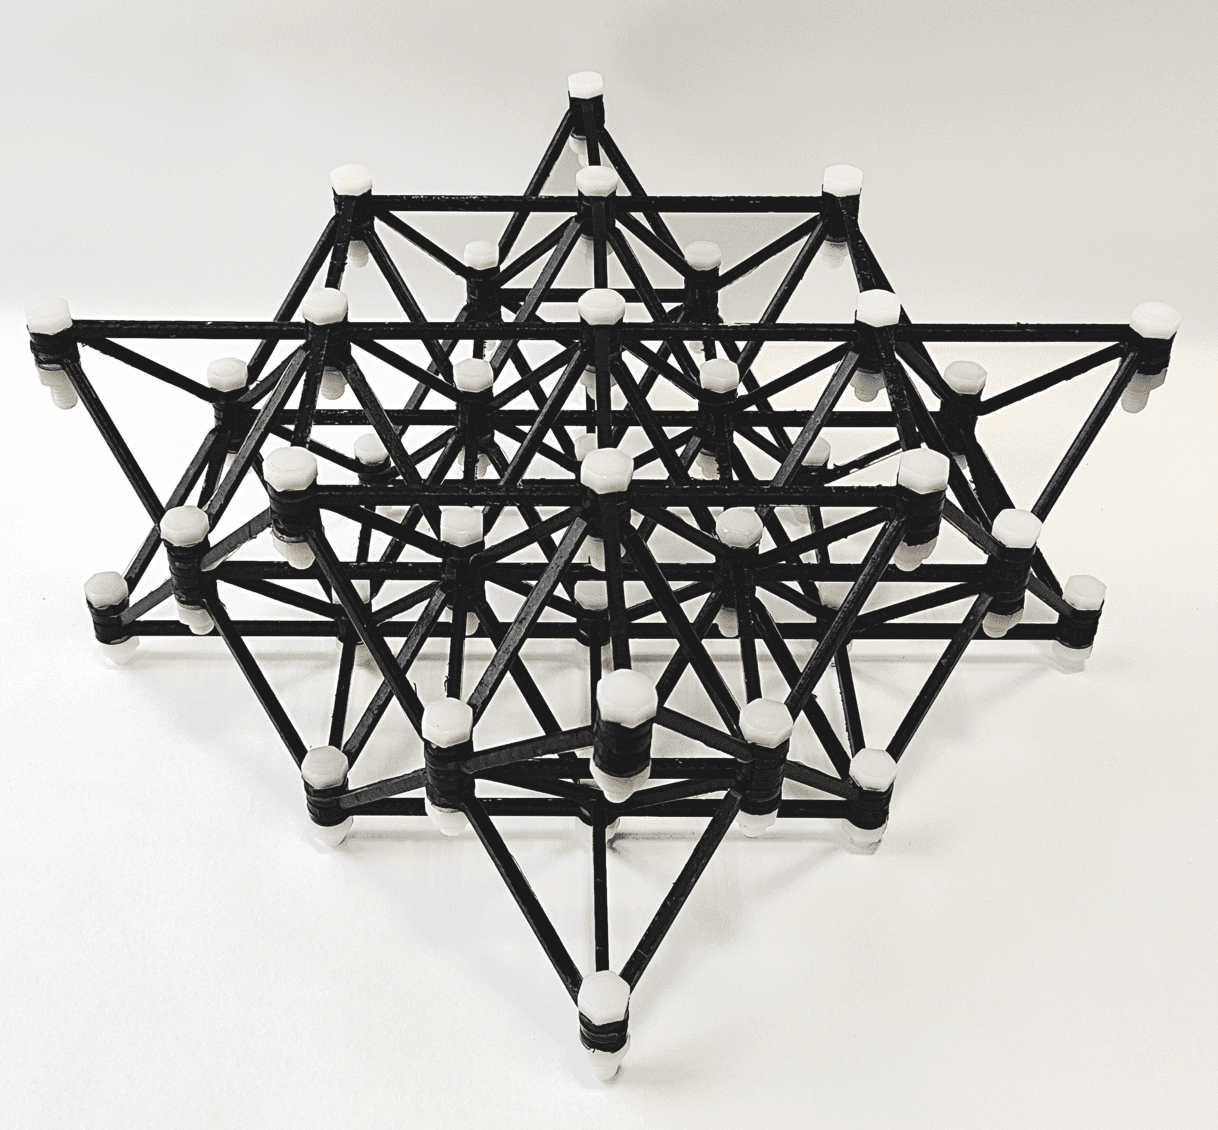
\includegraphics[width=\linewidth]{figures/01_intro/starac.png}
    \caption{Example of a reversibly assembled modular lattice structure made by \gls{cfrp} using the \gls{tfp} technology built for mechanical testing at ONERA in the STARAC research project.}
    \label{fig:01_starac}
\end{marginfigure}

\section*{Objective}
Optimizing modular lattice structures involves four main dimensions: material, module shape, layout, and topology. Material optimization focuses on improving mechanical properties by tailoring the material distribution within lattice constituents, while shape optimization fine-tunes the repeating module geometry. Layout optimization arranges modules in space, defining their presence or absence in the design region, and topology optimization refines the overall arrangement and connections of bars within each module. Navigating these dimensions enables engineers to tailor lattice structures for a balance between weight, strength, and functionality. However, the abundance of design choices poses a significant challenge due to the lack of an optimized design method. Using available tools, it is possible to create oversized structures using modern robotic means. However, achieving better results is complex and requires leveraging numerical optimization tools to explore the design space. It is these tools, and even more importantly, the necessary methods, that are lacking. Thus, the challenge of this research lies not in designing modular lattice structures, but rather in realizing their full potential.

This thesis aims to develop an optimization methodology tailored for lightweight and modular aerospace structures. The methodology development involves working on problem formulation, theorize a resolution method, implementing it numerically, and validating the results against existing literature. The aim of the thesis is broad and complex, involving several interrelated subproblems. Initially, the focus is on optimizing lattices without modularity while considering mechanical failure constraints. Subsequently, attention shifts to incorporating modularity into the optimization process and assessing its impact on mass and performance. Further, efforts are directed towards optimizing the arrangement of repeating modules alongside their individual designs. Finally, the methodology is extended to the scale of a full wing for aerospace applications.


\section*{Outline of the thesis}
\chpref{chap:02} provides a review of structural optimization algorithms, especially focusing on ultralight weight and modular cases. The chapter introduces the density-based topology optimization and the \gls{tto} methods that will be utilized throughout the document. \chpref{chap:03} presents two equivalent volume minimization formulations: one for density-based topology optimization and another for the \gls{tto} method. It then conducts an in-depth comparison of the resulting optimized structures, focusing on those with volume fractions below \qty{5}{\percent}. The numerical analysis reveals shorter computational times and improved performance with the \gls{tto} approach, particularly in modeling lightweight structures. For these reason, the \gls{tto} approach is selected. \chpref{chap:04} introduces additional features with respect to the classic \gls{tto} formulation, such as local buckling constraints, minimum slenderness limits, consideration of multiple load cases, and ensuring mechanical compatibility for complex structures. Some of these constraints have been already studied in the literature, but they have never been considered in a single comprehensive volume minimization formulation. Due to the inherent multimodality of the problem, a two-step optimization algorithm is introduced, utilizing a relaxed problem to generate an initial approximate solution for subsequent optimization using a complete non-linear formulation. In an effort to minimize the impact of the initial starting point on optimization outcomes, a heuristic is formulated to reintroduce candidates into the optimization process when it converges to local minima. \chpref{chap:05} explores how to formulate a modular optimization problem within the \gls{tto} framework, employing the full-scale variable linking approach. This approach optimizes the topology of a single module that is repeated throughout the entire design region to create modular structures. The chapter evaluates the impact of hyperparameters, such as the number of subdomains and the choice of the module ground structure, on the mechanical performance of the structure. A \gls{doe}, based on the chapter's results, helps to formulate a guide on choosing hyperparameters for optimization. In \chpref{chap:06} we complicate the optimization by introducing multiple modules into the process. Each module is optimized independently, as well as the selection of the active module in each subdomain. A modified \gls{dmo} approach is proposed to solve the discrete optimization problem, utilizing a gradient-based optimizer, while the starting point is determined by employing k-means clustering on the stress distribution of the optimization starting point. In \chpref{chap:07} the proposed optimization methodologies are applied to more ambitious aerospace cases that require some minor methodological adaptations. First, the monolithic \gls{tto} algorithm is used to reduce the mass of the wingbox of the \gls{crm}, a standard benchmark for aeronautic research. The test case is subjected to real-world multiple load cases (+2.5g, -1g, and cruise maneuver loads) associated with some respective safety factors. The optimization is conducted using different materials and discretizations, resulting in lighter structures with less computational effort compared to the literature. Later, the modular formulation presented in \chpref{chap:06} is used on a drone-sized wing based on the 0012 NACA wing profile, validating the ability of the proposed modular optimization methodology to work on real-world test cases. Additionally, follow-up scientific perspectives are discussed.